\subsubsection{Determinación de umbrales y validación}

Construcción del dataset.\\
\noindent
Se construyó un dataset representativo mediante captura de imágenes bajo condiciones operativas reales. El dataset incluyó lechugas en diferentes estados de desarrollo (desde plántulas hasta plantas maduras listas para cosecha) y vasos vacíos, bajo diferentes condiciones de iluminación dentro del rango operativo del invernadero.

\begin{figure}[H]
    \centering
    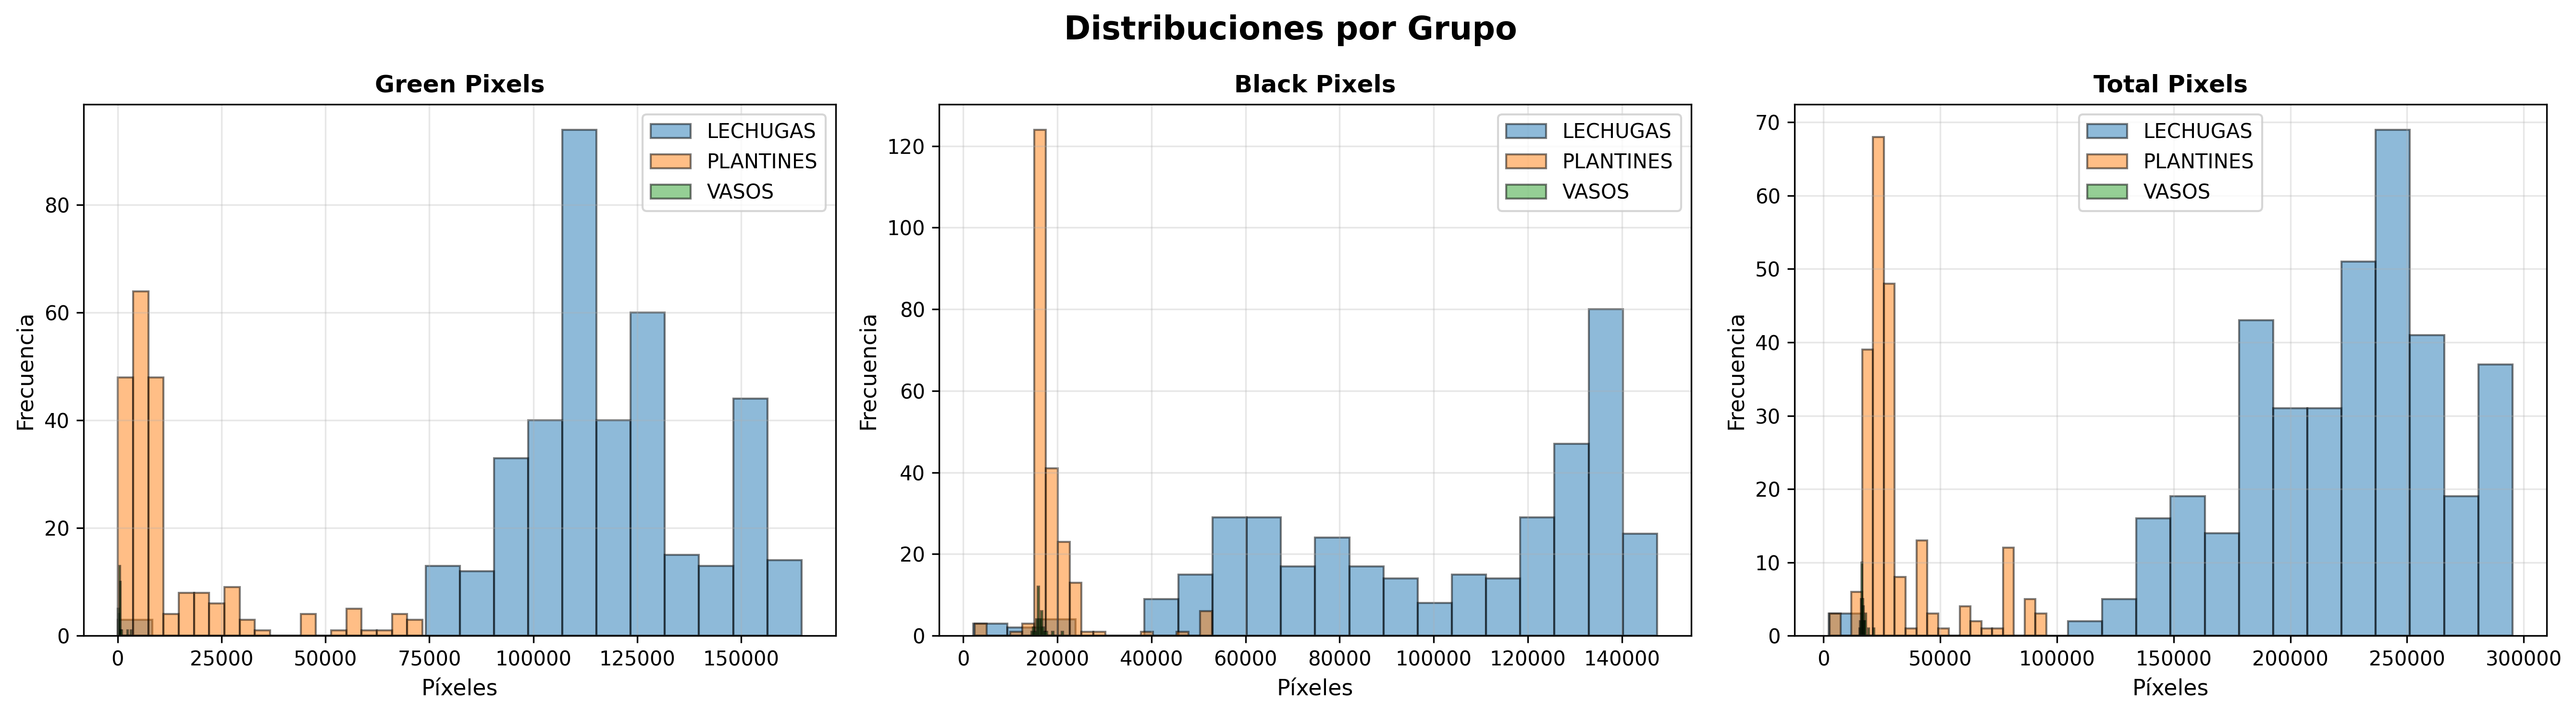
\includegraphics[width=0.6\textwidth]{img/distribuciones.png}
    \caption{Estadísticas de los grupos: lechugas, plantines y vasos.}
    \label{fig:distribuciones}
\end{figure}

Análisis estadístico.\\
\noindent
Para cada imagen se ejecutó el algoritmo de detección y se registró el área del contorno principal identificado. Los datos se analizaron estadísticamente para cada clase por separado, revelando separación clara entre las distribuciones de áreas de lechugas maduras y vasos vacíos/plantas inmaduras.

El análisis reveló que el descriptor de área presenta alto poder discriminativo. La diferencia significativa entre las medias de ambas clases, combinada con dispersiones relativamente pequeñas, indica que las distribuciones presentan solapamiento mínimo.\\

Umbral de clasificación.\\
\noindent
El umbral óptimo se determinó como el punto que minimiza la probabilidad total de error de clasificación. Este umbral define la frontera de decisión: muestras con área mayor o igual se clasifican como lechuga madura lista para cosecha, y muestras con área inferior se clasifican como planta inmadura o vaso vacío.

Se define además una zona de incertidumbre alrededor del umbral donde las clasificaciones reciben un índice de confianza reducido. Muestras fuera de esta zona reciben alta confianza. Esta información de confianza permite al nivel supervisor implementar estrategias de verificación adicional cuando sea necesario.\\

Validación experimental.\\
\noindent
El sistema se validó con un conjunto de prueba independiente que no participó en el establecimiento de los parámetros. Los resultados demuestran que el clasificador alcanza precisión adecuada para la aplicación, con errores principalmente en casos de plantas en estado muy temprano de desarrollo que normalmente no se cosecharían.
